\documentclass[uplatex,dvipdfmx,titlepage]{jsarticle}
\usepackage[dvipdfmx]{graphicx}
\usepackage{amsmath,amssymb}
\usepackage{bm}
\usepackage{enumitem} 
\usepackage{float}

%レポート作成に関する注意
%レポートには実験の目的、内容、実験方法、実験結果、結果に関する吟味・考察、予想との乖離があるならその原因の考察を自分の言葉でまとめる

\title{固体力学の実験}
\author{京都大学工学部物理工学科 1025363386 伊藤温大}
\date{\today}

\begin{document}
\maketitle
\section{はじめに}
本レポートでは超音波計測による弾性波伝搬速度と弾性係数の評価についてその結果、実験課題について報告する。

\section{超音波計測による弾性波伝搬速度と弾性係数の評価}
%間違いがないかどうか調べる。
\section{実験原理：超音波による弾性係数の評価}

固体中を伝搬する弾性波の速度は、材料の密度と弾性係数に依存する。本実験では、縦波および横波の伝搬速度を計測することで、材料のヤング率 $E$ およびポアソン比 $\nu$ を評価する。

\subsection{弾性波の伝搬速度}
等方性弾性体中を伝搬する縦波（疎密波）の速度 $c_L$ および横波（せん断波）の速度 $c_T$ は、材料の密度を $\rho$、ラメの定数を $\lambda, \mu$ とすると以下の式で表される。

\begin{equation}
    c_L = \sqrt{\frac{\lambda + 2\mu}{\rho}}
\end{equation}
\begin{equation}
    c_T = \sqrt{\frac{\mu}{\rho}}
\end{equation}

ここで、$\mu$ は剛性率である。これらの速度比から、ポアソン比 $\nu$ を以下の関係式によって導出できる。

\begin{equation}
    \nu = \frac{c_L^2 - 2c_T^2}{2(c_L^2 - c_T^2)}
\end{equation}

また、ヤング率 $E$ は、剛性率 $\mu$ とポアソン比 $\nu$ を用いて次のように算出される。

\begin{equation}
    E = 2\mu(1 + \nu) = 2\rho c_T^2(1 + \nu)
\end{equation}

\subsection{Rayleigh波の特性}
材料の表面に沿って伝搬する Rayleigh 波の速度 $c_R$ は、縦波および横波の速度を用いて以下の近似式（Viktorovの式）で表される。

\begin{equation}
    c_R \approx \frac{0.87 + 1.12\nu}{1 + \nu} c_T
\end{equation}

本実験では、トランスデューサ間の間隔を変化させて到達時刻を測定し、実測値としての $c_R$ を算出することで、上記理論値との比較・検討を行う。
\subsection{実験方法}
\subsubsection*{実験1}
金属ブロックに縦波および、横波の超音波を送信、受信することによって測定波形から伝搬速度を求めた。
\begin{itemize}[nosep]
    \item 超音波送受信装置
    \item トランスデューサー
    \item 音響結合媒質
    \item 試験片
    \item ディジタルオシロスコープ
    \item パーソナルコンピューター
\end{itemize}
具体的に試験片として以下の材料を用いた。
\begin{itemize}[nosep]
    \item 機械構造用炭素鋼鋼材 S25C
    \item 機械構造用炭素鋼鋼材 S45C
    \item アルミニウム合金 A5052
    \item アルミニウム合金 A2024(超ジュラルミン)
\end{itemize}
この際、以下のような実験手順を実施した。

\begin{enumerate}[label=\arabic*.]
    \item 試験片の寸法を測定し、記録した。この時同様の材質について4回測定し、平均をとった。記録した試験片の寸法は以下の表のようになった。
    \begin{table}[H]
        \centering
        \begin{tabular}{lccc}
        \hline
        S25C & S45C & A5052 & A2025 \\ \hline
        9.882 & 9.873 & 9.98 & 10.061 \\ \hline
        \end{tabular}
    \end{table}

    \item 試験片を厚さ方向に複数回伝搬した波形について、それぞれの反射波の到着時刻を求めた。この時S25Cの縦波について初めの波は超音波送受信装置から出た波を観測してしまっていると考えられる。
    \item このとき縦波については5MHZ,横波については1MHZの波を発生させた。
    \item 受信した反射波形に含まれる周波数成分を、高速フーリエ変換を行うことによって確認した。\\
    この際以下の手順を行った。
    \begin{itemize}
        \item 受信波形のうち、単一パルスだけを対象とし、他のエコーを表すデータはすべて0に置き換えた。また時間データ数が2のべき乗となるように必要な個数だけ末尾に0データを加えた。
        \item このデータに対して高速フーリエ変換を行い、結果として出力される複素数について絶対値を計算しグラフ化した。この際データの周波数間隔はテキスト(4-6)の式によって求めた。
        \begin{equation}
        \Delta f = \frac{f_s}{N} = \frac{1}{NT_s} = \frac{1}{T}
        \end{equation}
    \end{itemize}
    今回はA2024の縦波、A2024の横波それぞれについて高速フーリエ変換を行った。
\end{enumerate}

\subsubsection*{実験2}
送信トランスデューサと受信トランスデューサの間隔を変化させながら、波の到達時刻を調べた。
この時送信トランスデューサと受信トランスデューサの間隔は2, 4, 6, 8 cmについてそれぞれ波の到達時刻を調べた。

% --------------------------------------------------
\subsection{実験結果}
% --------------------------------------------------
% TO DO 縦波と横波の理論値との相対誤差との比較?<-無理そう。どっちかというとE,νの相対誤差の比較？
\subsubsection*{実験1の測定結果}
縦波について、受信したデータはS25Cから順に以下図のようになった。
\begin{figure}[H]
    \centering
    \begin{minipage}[b]{0.48\textwidth}
        \centering
        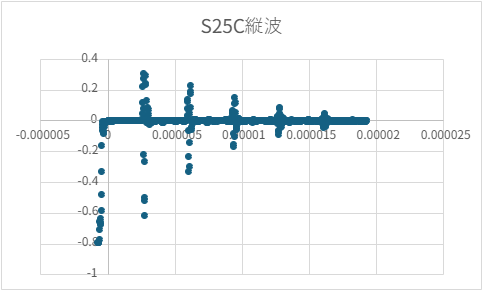
\includegraphics[width=\textwidth]{S25C縦波.png}
        \caption{S25C 縦波}
    \end{minipage}
    \hfill
    \begin{minipage}[b]{0.48\textwidth}
        \centering
        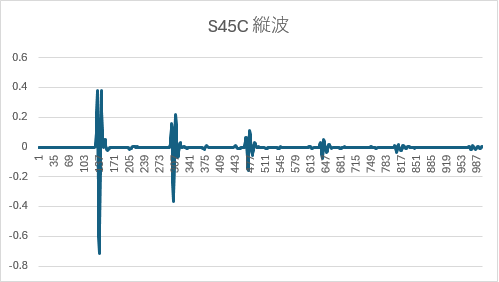
\includegraphics[width=\textwidth]{S45C縦波.png}
        \caption{S45C 縦波}
    \end{minipage}
    \\ \vspace{5mm}
    \begin{minipage}[b]{0.48\textwidth}
        \centering
        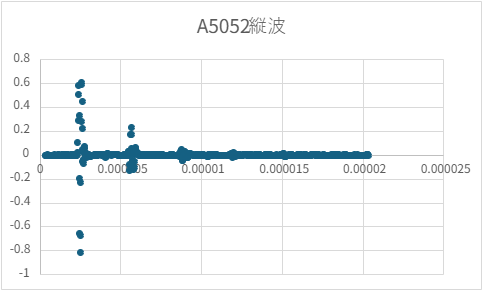
\includegraphics[width=\textwidth]{A5052縦波.png}
        \caption{A5052 縦波}
    \end{minipage}
    \hfill
    \begin{minipage}[b]{0.48\textwidth}
        \centering
        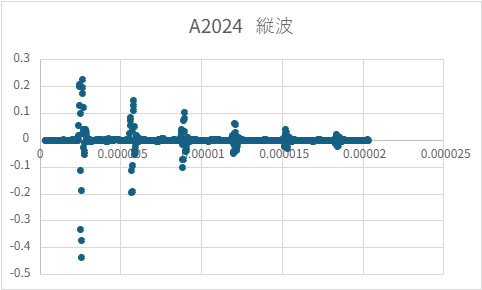
\includegraphics[width=\textwidth]{A2024縦波.png}
        \caption{A2024 縦波}
    \end{minipage}
\end{figure}

この反射波の到着時刻を求める際には波の下限のピークの値を到着時刻として統一した。この時縦波における到着時刻はS25Cから順に以下の表のようになった。
\begin{table}[H]
    \centering
    \caption{S25C 縦波の到着時刻}
    \begin{tabular}{lcc}
    \hline
    個数 & 到着時刻 & 総距離 \\ \hline
    1つ目 & 0.00000274 & 0.019764 \\
    2つ目 & 0.00000606 & 0.039528 \\
    3つ目 & 0.0000094  & 0.059292 \\
    4つ目 & 0.00001272 & 0.079056 \\
    5つ目 & 0.00001606 & 0.09882  \\ \hline
    \end{tabular}
\end{table}

\begin{table}[H]
    \centering
    \caption{S45C 縦波の到着時刻}
    \begin{tabular}{lcc}
    \hline
    個数 & 到着時刻 & 総距離 \\ \hline
    1つ目 & 0.00000274 & 0.019746 \\
    2つ目 & 0.00000608 & 0.039492 \\
    3つ目 & 0.00000944 & 0.059238 \\
    4つ目 & 0.00001278 & 0.078984 \\ \hline
    \end{tabular}
\end{table}

\begin{table}[H]
    \centering
    \caption{A5052 縦波の到着時刻}
    \begin{tabular}{lcc}
    \hline
    個数 & 到着時刻 & 総距離 \\ \hline
    1つ目 & 0.0000025  & 0.01996 \\
    2つ目 & 0.00000558 & 0.03992 \\
    3つ目 & 0.00000884 & 0.05988 \\ \hline
    \end{tabular}
\end{table}

\begin{table}[H]
    \centering
    \caption{A2024 縦波の到着時刻}
    \begin{tabular}{lcc}
    \hline
    個数 & 到着時刻 & 総距離 \\ \hline
    1つ目 & 0.00000264 & 0.020122 \\
    2つ目 & 0.00000578 & 0.040244 \\
    3つ目 & 0.00000892 & 0.060366 \\
    4つ目 & 0.00001206 & 0.080488 \\
    6つ目 & 0.0000152  & 0.10061  \\
    7つ目 & 0.0000185  & 0.120732 \\ \hline
    \end{tabular}
\end{table}

このとき伝搬速度は以下の表のようになった。(m/s)
\begin{table}[H]
    \centering
    \begin{tabular}{lccc}
    \hline
    S25C & S45C & A5052 & A2025 \\ \hline
    5935.1 & 5897.8 & 6294.8 & 6361.5 \\ \hline
    \end{tabular}
\end{table}

横波について、観測したオシロスコープの値は以下の図のようになった。
\begin{figure}[H]
    \centering
    \begin{minipage}[b]{0.48\textwidth}
        \centering
        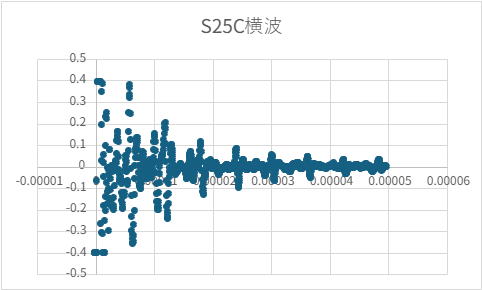
\includegraphics[width=\textwidth]{S25C横波.png}
        \caption{S25C 横波}
    \end{minipage}
    \hfill
    \begin{minipage}[b]{0.48\textwidth}
        \centering
        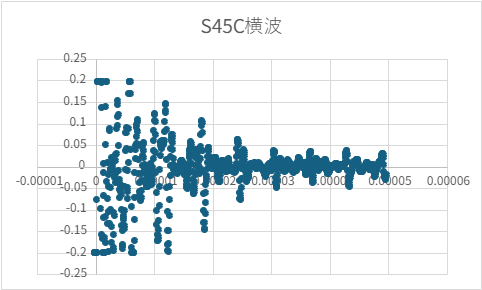
\includegraphics[width=\textwidth]{S45C横波.png}
        \caption{S45C 横波}
    \end{minipage}
    \\ \vspace{5mm}
    \begin{minipage}[b]{0.48\textwidth}
        \centering
        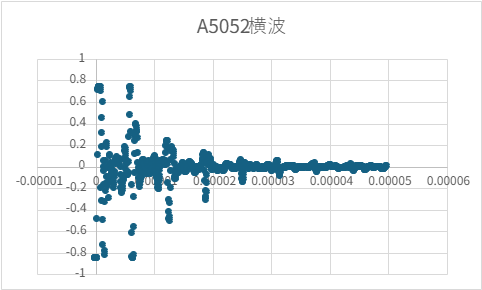
\includegraphics[width=\textwidth]{A5052横波.png}
        \caption{A5052 横波}
    \end{minipage}
    \hfill
    \begin{minipage}[b]{0.48\textwidth}
        \centering
        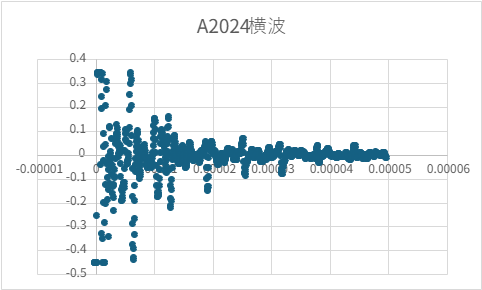
\includegraphics[width=\textwidth]{A2024横波.png}
        \caption{A2024 横波}
    \end{minipage}
\end{figure}

到着時刻はS25Cから順に以下の表のようになった。この際、1, 2回目などの波が不安定になっている点については考慮せず、安定に観測できている波について観測した。この時横波における到着時刻は波の下限のピークの値を到着時刻として統一した。

\begin{table}[H]
    \centering
    \caption{S25C 横波の到着時刻}
    \begin{tabular}{lcc}
    \hline
    個数 & 到着時刻 & 総距離 \\ \hline
    4つ目 & 2.45E-05 & 0.079056 \\
    5つ目 & 3.05E-05 & 0.09882  \\
    6つ目 & 3.67E-05 & 0.118584 \\
    7つ目 & 4.27E-05 & 0.138348 \\ \hline
    \end{tabular}
\end{table}

\begin{table}[H]
    \centering
    \caption{S45C 横波の到着時刻}
    \begin{tabular}{lcc}
    \hline
    個数 & 到着時刻 & 総距離 \\ \hline
    3つ目 & 1.86E-05 & 0.059238 \\
    4つ目 & 2.47E-05 & 0.078984 \\
    5つ目 & 3.1E-05  & 0.09873  \\
    6つ目 & 3.72E-05 & 0.118476 \\ \hline
    \end{tabular}
\end{table}

\begin{table}[H]
    \centering
    \caption{A5052 横波の到着時刻}
    \begin{tabular}{lcc}
    \hline
    個数 & 到着時刻 & 総距離 \\ \hline
    2つ目 & 6.25E-06 & 0.03992 \\
    3つ目 & 1.26E-05 & 0.05988 \\
    4つ目 & 1.88E-05 & 0.07984 \\ \hline
    \end{tabular}
\end{table}

\begin{table}[H]
    \centering
    \caption{A2024 横波の到着時刻}
    \begin{tabular}{lcc}
    \hline
    個数 & 到着時刻 & 総距離 \\ \hline
    2つ目 & 6.4E-06  & 0.040244 \\
    4つ目 & 1.91E-05 & 0.080488 \\
    5つ目 & 2.56E-05 & 0.10061  \\ \hline
    \end{tabular}
\end{table}

これによって伝搬速度は以下のようになった。
\begin{table}[H]
    \centering
    \begin{tabular}{lccc}
    \hline
    S25C & S45C & A5052 & A2024 \\ \hline
    3245.3 & 3189.9 & 3180.9 & 3154.6 \\ \hline
    \end{tabular}
\end{table}

実験1によって導かれる各材料のヤング率とポアソン比を求めると以下の表のようになった。
\begin{table}[H]
    \centering
    \begin{tabular}{lcc}
    \hline
    材料 & $E$ & $\nu$ \\ \hline
    S25C  & 211.4107036 & 0.286745546 \\
    S45C  & 205.2874965 & 0.293253799 \\
    A5052 & 75.27726346 & 0.328543453 \\
    A2024 & 74.50623148 & 0.336952484 \\ \hline
    \end{tabular}
\end{table}

高速フーリエ変換を行った結果は以下のようである。
\begin{figure}[H]
    \centering
    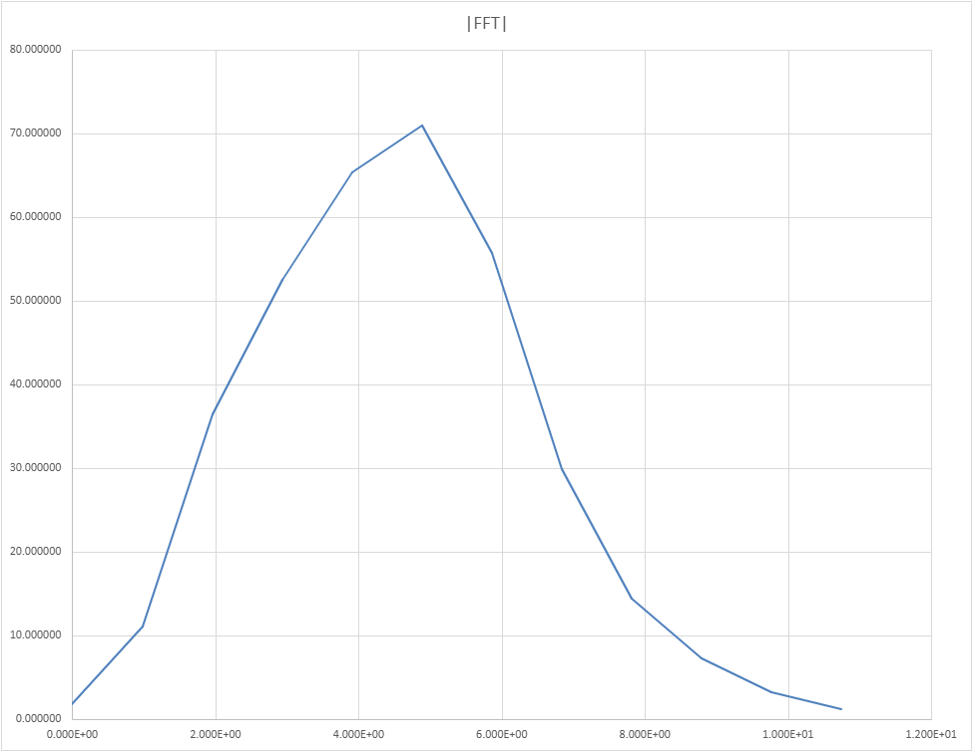
\includegraphics[width=12cm]{高速フーリエ変換A2024縦波.png}
    \caption{A2024縦波の高速フーリエ変換}
\end{figure}
\begin{figure}[H]
    \centering
    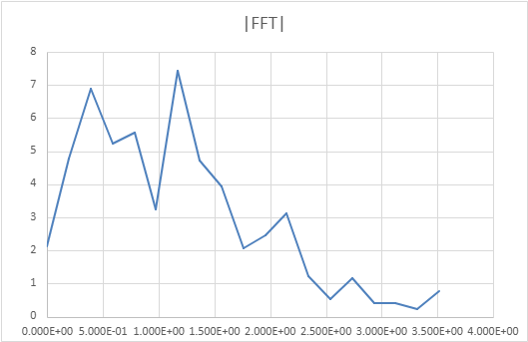
\includegraphics[width=12cm]{高速フーリエ変換A2024横波.png}
    \caption{A2024横波の高速フーリエ変換}
\end{figure}

\subsubsection*{実験2の測定結果}
この時観測した波の到達時刻は以下のようになった。
それぞれの材料におけるそれぞれの間隔の到達時刻は以下の表に示す。

\begin{table}[H]
    \centering
    \caption{S25C}
    \begin{tabular}{lc}
    \hline
    到達時刻 & 距離(m) \\ \hline
    0.00002215 & 0.02  \\
    0.0000287  & 0.04  \\
    0.0000352  & 0.06  \\
    0.0000422  & 0.08  \\ \hline
    \end{tabular}
\end{table}

\begin{table}[H]
    \centering
    \caption{S45C}
    \begin{tabular}{lc}
    \hline
    到達時刻 & 距離(m) \\ \hline
    0.00002175 & 0.02 \\
    0.00002835 & 0.04 \\
    0.0000348  & 0.06 \\
    0.00004215 & 0.08 \\ \hline
    \end{tabular}
\end{table}

\begin{table}[H]
    \centering
    \caption{A5052}
    \begin{tabular}{lc}
    \hline
    到達時刻 & 距離(m) \\ \hline
    0.0000225  & 0.02 \\
    0.00002915 & 0.04 \\
    0.00003615 & 0.06 \\
    0.00004275 & 0.08 \\ \hline
    \end{tabular}
\end{table}

\begin{table}[H]
    \centering
    \caption{A2024}
    \begin{tabular}{lc}
    \hline
    到達時刻 & 距離(m) \\ \hline
    2.27E-05 & 0.02 \\
    2.93E-05 & 0.04 \\
    3.62E-05 & 0.06 \\
    4.36E-05 & 0.08 \\ \hline
    \end{tabular}
\end{table}

トランスデューサ間の間隔と到達時刻との関係から求めた伝搬速度と、実験1における横波速度とPoisson比によるRayleigh波の速度との関係は以下のようになった。
\begin{table}[H]
    \centering
    \resizebox{\textwidth}{!}{
    \begin{tabular}{lccccc}
    \hline
          & Poisson比 & 横波速度 & Rayleigh波(実験1) & Rayleigh波(実測値) & 誤差(\%)  \\ \hline
    S25C  & 0.2868   & 3245.3 & 3004.238       & 2959.8         & 1.479173 \\
    S45C  & 0.2933   & 3189.9 & 2956.068       & 2953.9         & 0.073331 \\
    A5052 & 0.3285   & 3180.9 & 2964.019       & 2951           & 0.439247 \\
    A2024 & 0.337    & 3154.6 & 2943.287       & 2869.8         & 2.496754 \\ \hline
    \end{tabular}
    }
\end{table}

% --------------------------------------------------
\subsection{考察}
% --------------------------------------------------
高速フーリエ変換の結果よりA2024縦波においては5MHzにおいてピークをとっていることがわかる。
またA2024横波においては0.4, 1.1HZほどでピークを持っていることが分かる。
本実験については縦波については5MHZの波を発生させているため、おおよそ正しく解析できている。
一方でA2024においては実験装置において発生させた1.0MHZの波以外にも0.4MHZにもピークがあることがわかる。
この理由として本実験において波を伝達させるために音響結合媒質(カプラント)を用いているため波が減衰したと考えられる。
また本実験において横波については縦波より伝わりずらく減衰の影響がより強く出たと考えられる。

この実験結果から金属ブロックに超音波を当てることによってヤング率やポアソン比を求めることができた。
また実験1におけるRayleigh波と実測値としてのRayleigh波の誤差がおおよそ2\%以下であることから比較的良い精度で実験ができたといえる。

\subsubsection*{考察課題}
1. 超音波測定に用いた以下の4種類の材料に対して、ヤング率/密度として定義されている比剛性を求める。この際密度については
S25C, S45C = $7.8 \times 10^3$ kg$\cdot$m$^{-3}$ \\
A2024,A5052=$2.8 \times 10^3$ kg$\cdot$m$^{-3}$
いま文献[1]によるとそれぞれの材質について引張強さは以下のようになった。
\begin{table}[H]
\begin{tabular}{lll}
      & 引張強さ(kgf/mm\textasciicircum{}2) & 引張強さ(MPa) \\
S25C  & 45                              & 405       \\
S45C  & 58                              & 568.4     \\
A5052 & 24                              & 216       \\
A2024 & 44                              & 431.2    
\end{tabular}
\end{table}
よって比剛性、比強度は計算すると以下のようになった。
\begin{table}[H]
\begin{tabular}{lllll}
      & 比剛性      & ヤング率(GPa)   & 引張強さ(MPa)  & 比強度(MPa/(g/cm$^3$))    \\
S25C  & 2.710394 & 211.4107 & 405   & 5.192308 \\
S45C  & 2.631891 & 205.2875 & 568.4 & 7.287179 \\
A5052 & 2.688474 & 75.27726 & 216   & 7.714286 \\
A2024 & 2.660937 & 74.50623 & 431.2 & 15.4    
\end{tabular}
\end{table}
この結果からすべての材質について比剛性が同じようであった。つまり質量当たりの変形しやすさに違いはほぼない。
一方で比強度についてはA2024が他と2倍以上の差をつけて大きくなっている。つまり質量当たりの強度としてはA2024が秀でている。
以上よりこの4つの材料のうち航空機・宇宙機などの軽量構造には軽量でより強い強度を実現できるという点でA2024が最もいいといえる。\\
2. 超音波測定に用いた炭素鋼S25CとS45Cの違い、およびアルミニウム合金A5052とA2024の違いは参考文献[1]によるとそれぞれの材質について引張強さは以下のようになった
\begin{itemize}
    \item S25CとS45Cの違い
    \begin{itemize}
        \item S25C:炭素を約0.25\%含んでおり、切削加工性・鍛造性・鋳型性が良い。またボルト、ナット、ビスなどの大量生産部品に適している
        \item S45C:炭素を約0.45\%含んでおり、強さと粘り強さをを重視する部品に使用する:車軸、クランク軸
    \end{itemize}
    \item A5052とA2024の違い
    \begin{itemize}
    \item A5052:固溶化処理・時効硬貨処理は基本的には不要で冷間加工により強度を調整する。
    \item A2024:時効硬化処理が必要で焼入れ処理が重要である。
    \end{itemize}
\end{itemize}

\section{総括}
本実験を通して、光弾性法および超音波計測を用いた固体力学の評価手法について...

\begin{thebibliography}{99}
    \bibitem{jsme} 日本機械学会 編, 『機械工学便覧』, 丸善出版, pp. 2-21, 5-14, 5-19--5-20, 5-60.
\end{thebibliography}
\end{document}